%
%
%   ReQuiz 13A : 2022--04--27 (W)
%
%

\section{Exercise}

% Reference : SHW
% Graphing tool : https://www.desmos.com/calculator

(4 pt) Let $f : \reals \rightarrow \reals$ be the piecewise function, graphed below, whose rule of assignment is
\begin{align*}
f(x)
=
\begin{dcases*}
-x - 1			&	if $x \leq 0$		\\
-\sqrt{1 - x^{2}}	&	if $0 \leq x \leq 1$	\\
2 x - 2		&	if $x \geq 1$
\end{dcases*}
\end{align*}
This exercise explores the signed area under the graph of $f$ from $x = -3$ to $x = 3$.
\begin{center}
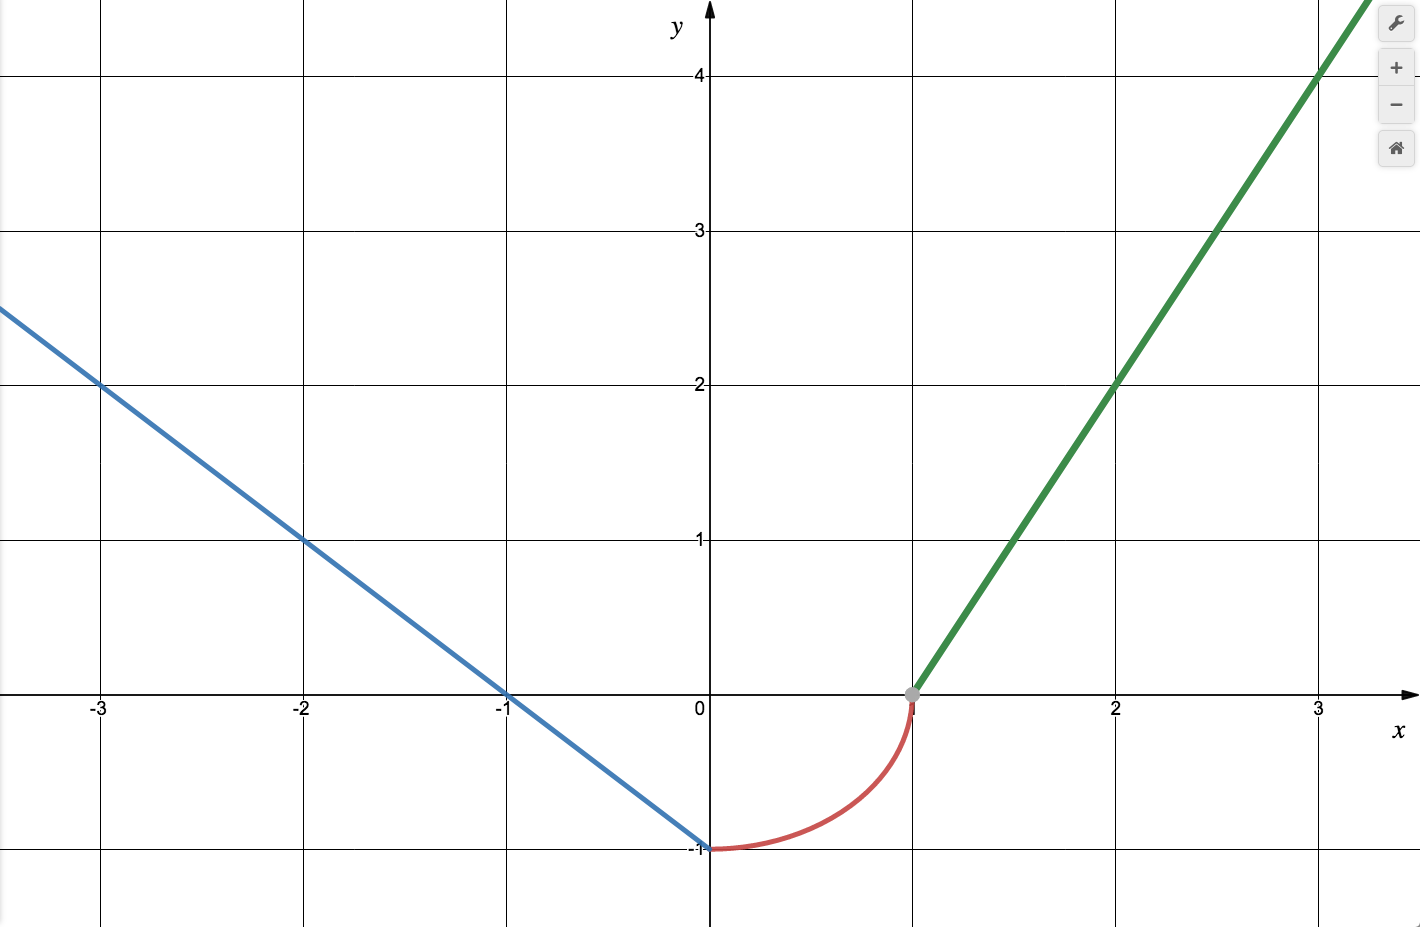
\includegraphics[width=0.35\textwidth]{\filePathGraphics/RQ13A_Graph.png}% Activate for quiz.
%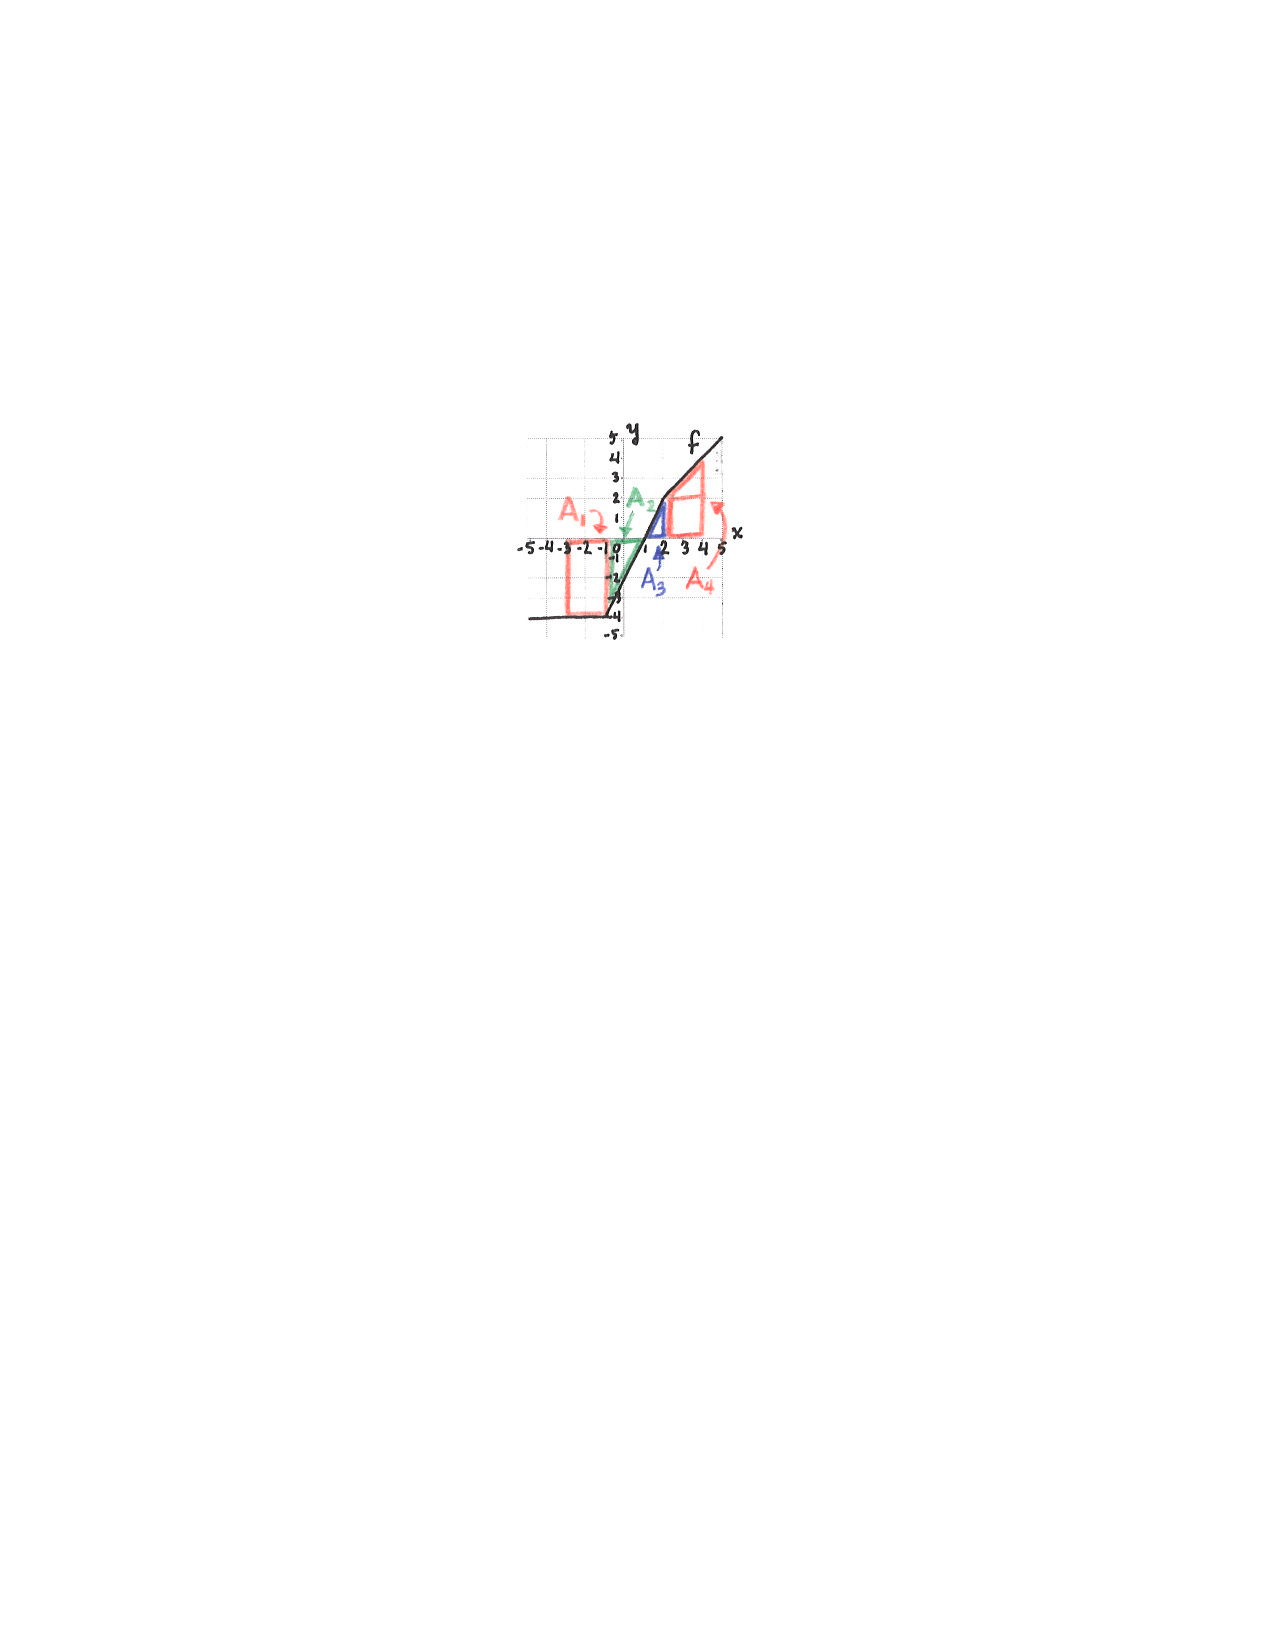
\includegraphics[scale=0.8]{\filePathGraphics/LQ13_Graph_Geometry.pdf}% Activate for solutions.
\end{center}



\begin{enumerate}[label=(\alph*)]
\item\label{itm : RQ13Aa} (1 pt) Use geometry to show that $\int_{-3}^{3} f(x) \spaceIntd \intd x = \frac{22 - \pi}{4} \approx 4.71$.
\end{enumerate}

\spaceSolution{1in}{% Begin solution.
}% End solution.



\begin{enumerate}[resume,label=(\alph*)]
\item\label{itm : RQ13Ab} (1 pt) On separate graphs below, draw a lower sum and an upper sum, each with six intervals of width $1$, to estimate $\int_{-3}^{3} f(x) \spaceIntd \intd x$. Show that $L \leq \int_{-3}^{3} f(x) \spaceIntd \intd x \leq U$.
\begin{center}
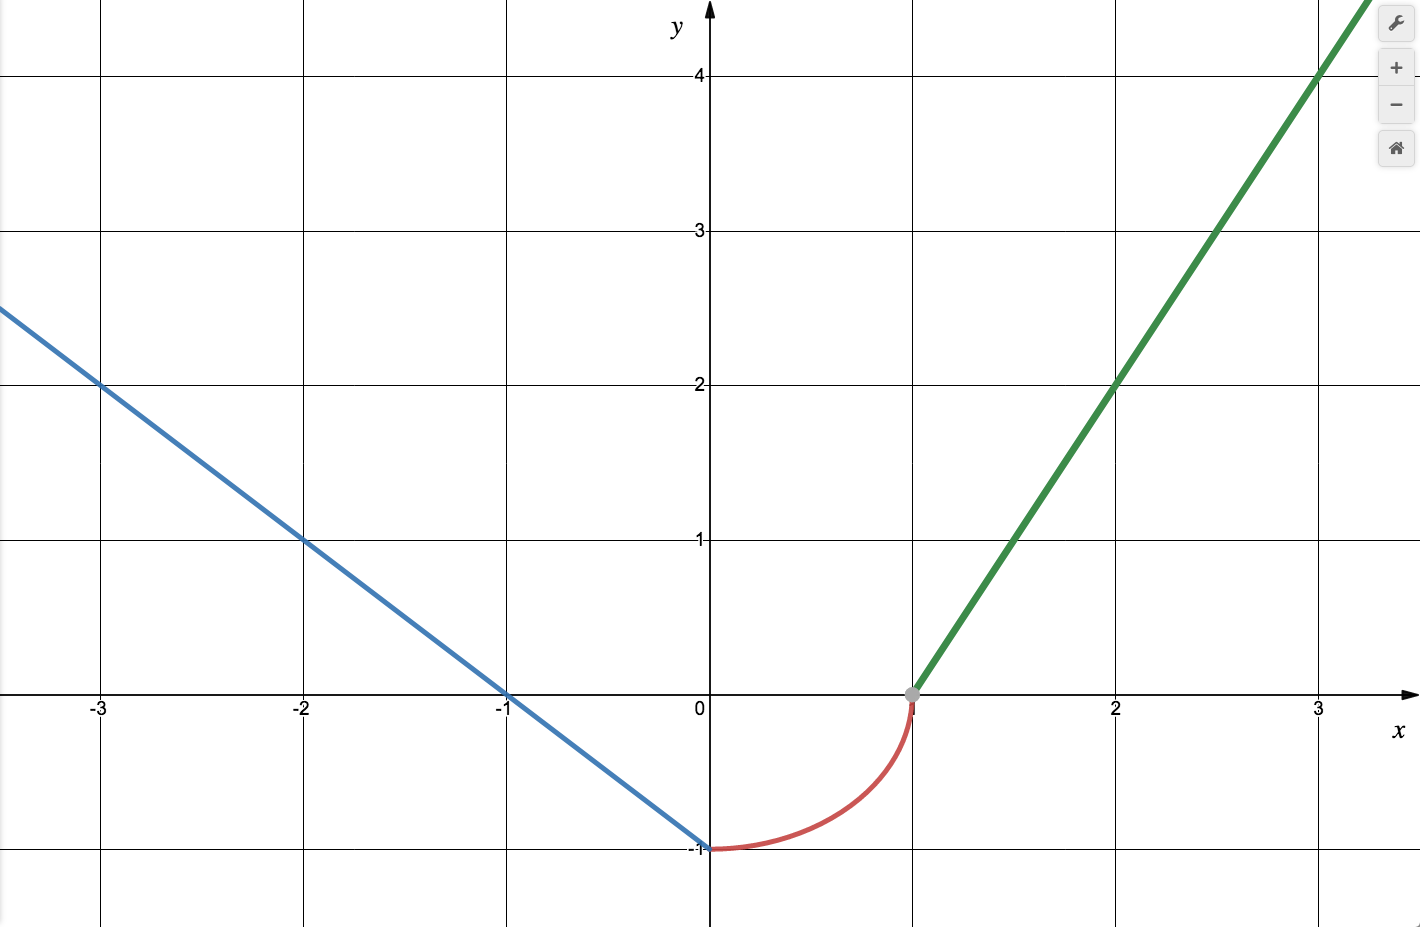
\includegraphics[width=0.35\textwidth]{\filePathGraphics/RQ13A_Graph.png}% Activate for quiz.
%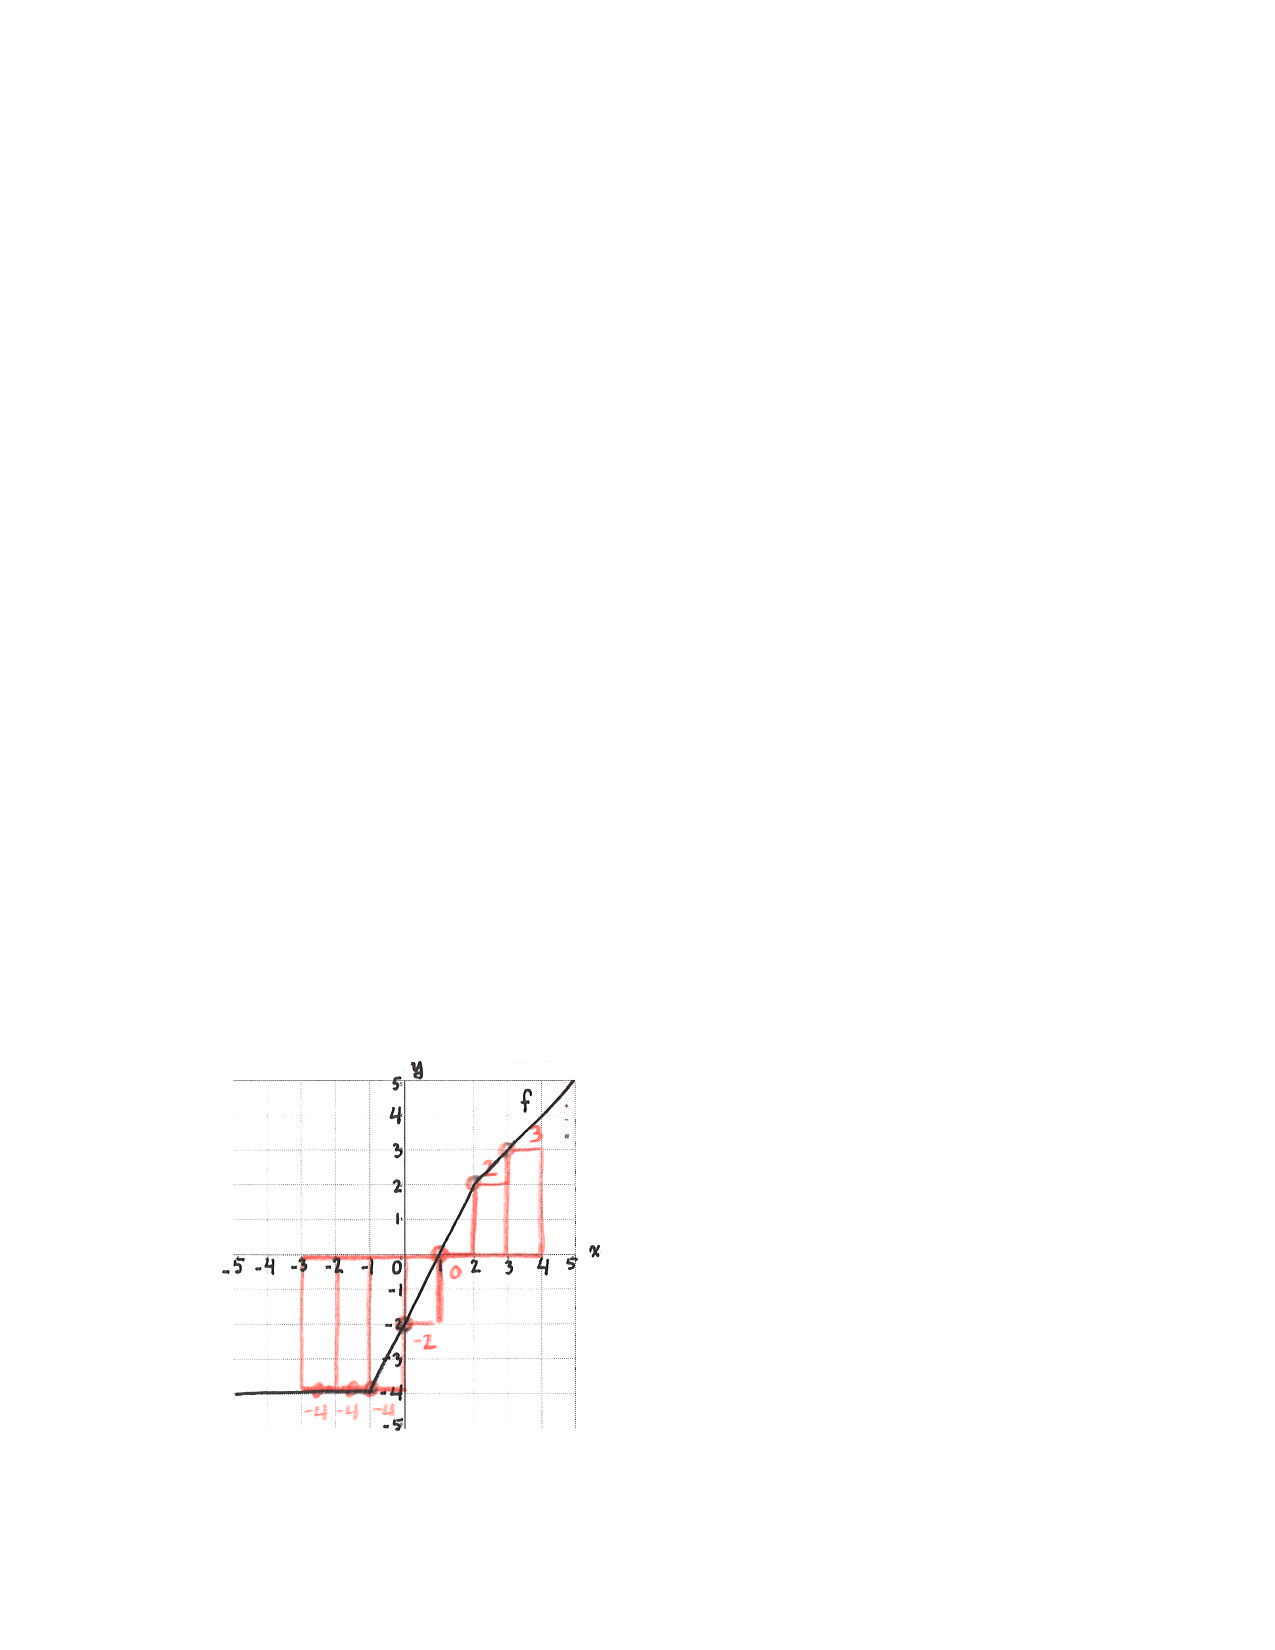
\includegraphics[scale=0.8]{\filePathGraphics/LQ13_Graph_Lower.pdf}% Activate for solutions.
\hspace{1in}
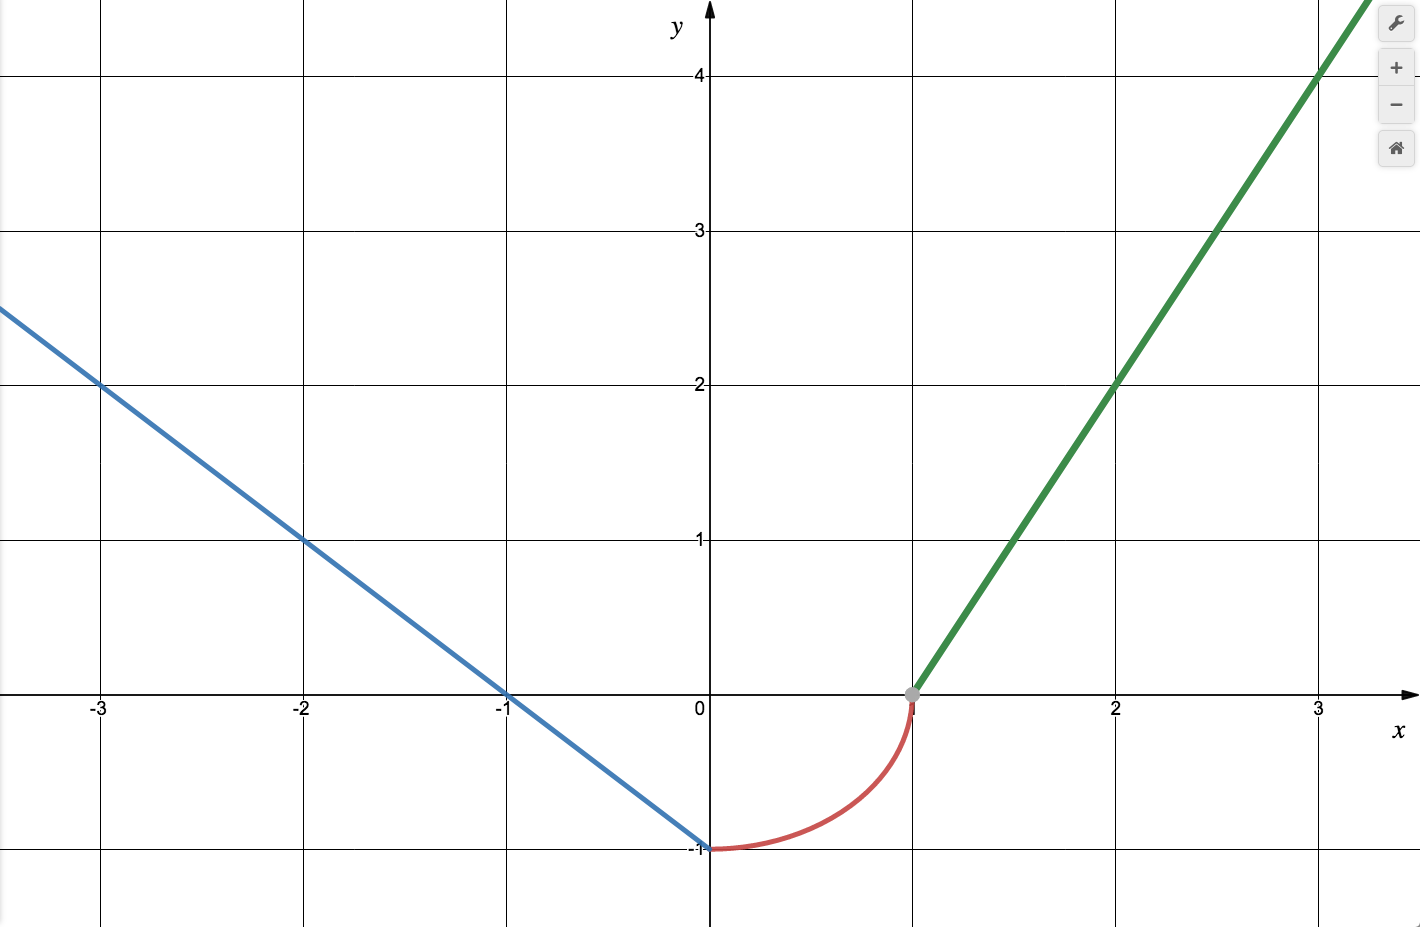
\includegraphics[width=0.35\textwidth]{\filePathGraphics/RQ13A_Graph.png}% Activate for quiz.
%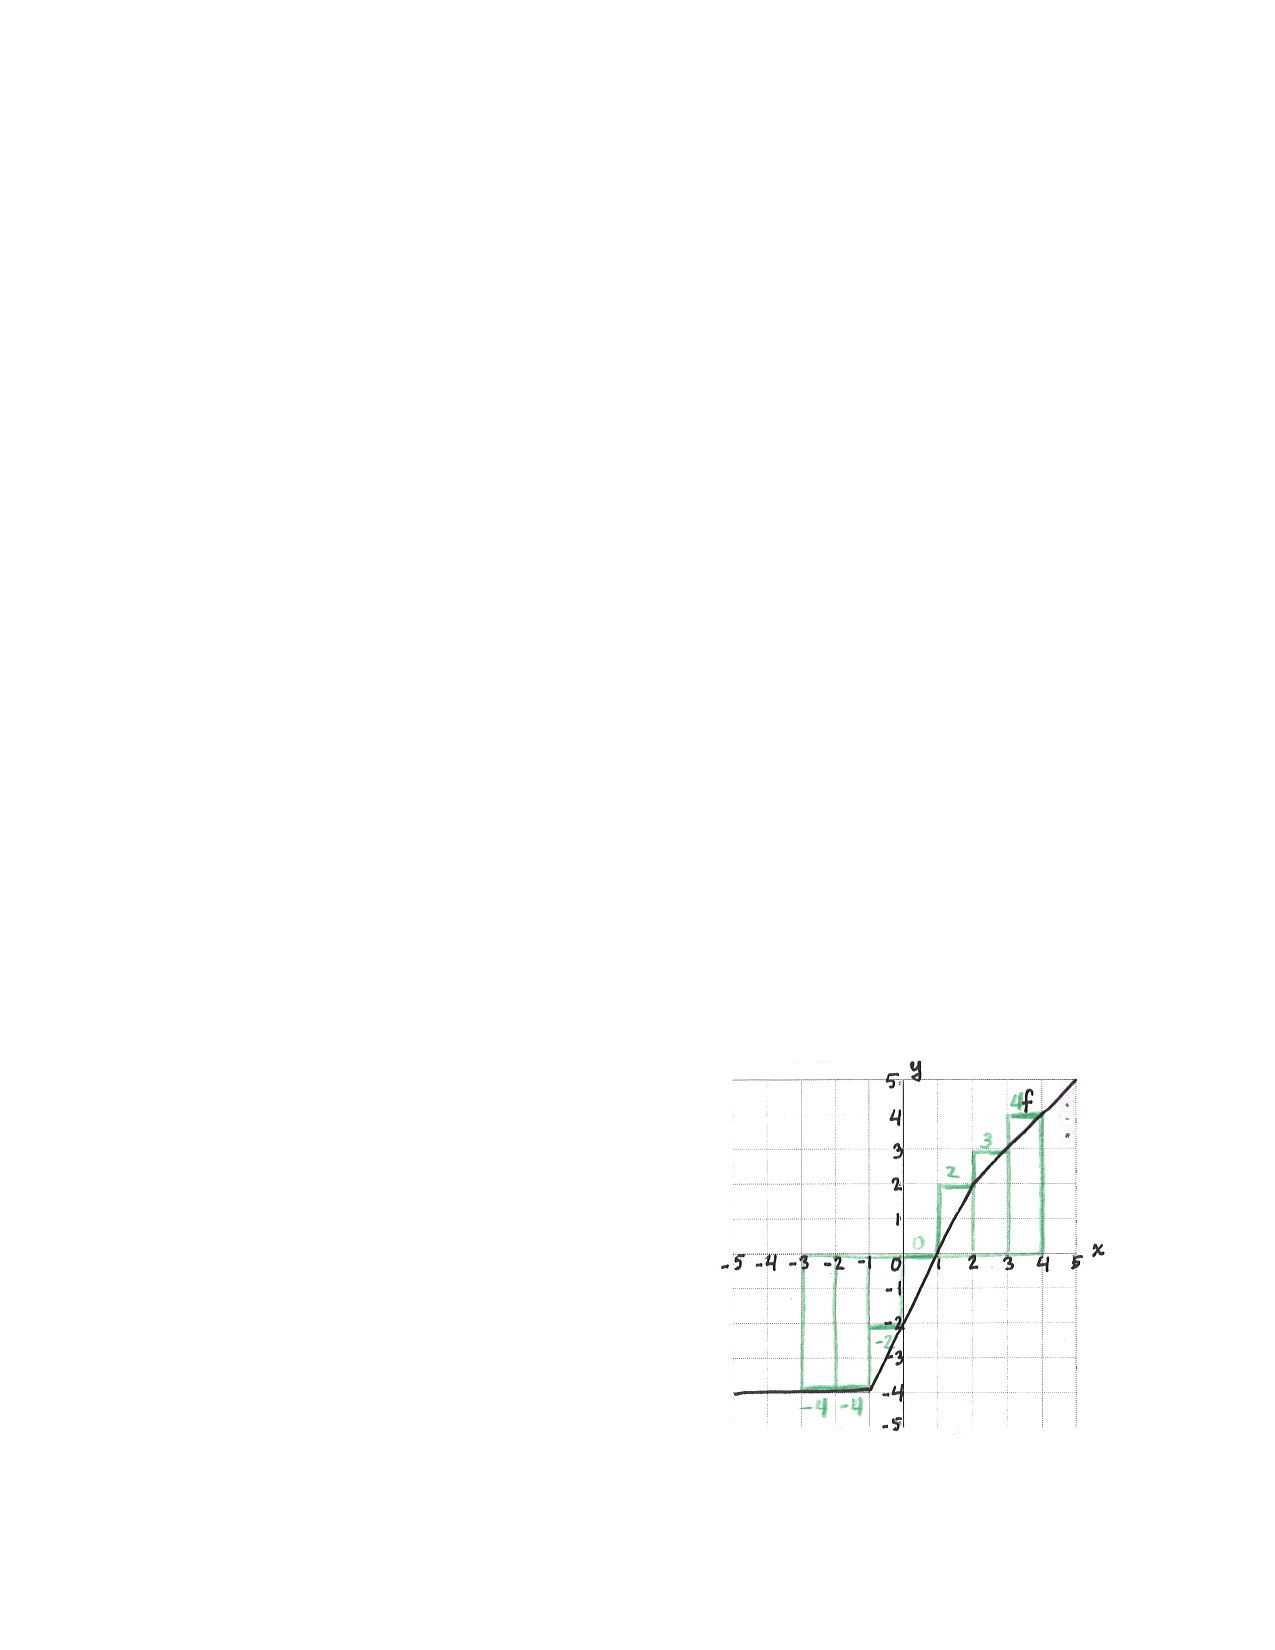
\includegraphics[scale=0.8]{\filePathGraphics/LQ13_Graph_Upper.pdf}% Activate for solutions.
\\
Lower sum ($L$)
\hspace{2.3in}
Upper sum ($U$)
\end{center}
\end{enumerate}

\spaceSolution{1in}{% Begin solution.
}% End solution.



\noindent{}For reference, $f : \reals \rightarrow \reals$ is the piecewise function whose rule of assignment is
\begin{align*}
f(x)
=
\begin{dcases*}
-x - 1			&	if $x \leq 0$		\\
-\sqrt{1 - x^{2}}	&	if $0 \leq x \leq 1$	\\
2 x - 2		&	if $x \geq 1$
\end{dcases*}
\end{align*}

\begin{enumerate}[resume,label=(\alph*)]
\item\label{itm : RQ13Ac} (2 pt) Find an antiderivative $F_{i}(x)$ for each ``piece'' $f_{i}(x)$ of $f(x)$. You may take as given that
\begin{align*}
\int -\sqrt{1 - x^{2}} \spaceIntd \intd x
=
-\frac{1}{2} \sin^{-1}(x) - \frac{1}{2} x \sqrt{1 - x^{2}} + C
\end{align*}
Use these antiderivatives $F_{i}(x)$ and the fundamental theorem of calculus to compute the value of each integral on the right side of the following equation:
\begin{align*}
\int_{-3}^{3} f(x) \spaceIntd \intd x
=
\int_{-3}^{0} f(x) \spaceIntd \intd x
+
\int_{0}^{1} f(x) \spaceIntd \intd x
+
\int_{1}^{3} f(x) \spaceIntd \intd x%
%\label{eq : RQ13A Piecewise Integral}
\end{align*}
Add your values for the three integrals on the right, and compare the result to part \ref{itm : RQ13Aa}.
\end{enumerate}

\spaceSolution{3in}{% Begin solution.
}% End solution.
